%%% Wähle zwischen 16:9 und 4:3 Format
\documentclass[aspectratio=169]{beamer} % 16:9
% \documentclass{beamer} % 4:3

\usepackage[ngerman]{babel} % Deutsche Sprache
\usepackage[utf8]{inputenc}
\usepackage{tikz}
\usepackage{graphicx}
\usepackage{array}
\usepackage{booktabs}

\usetheme{aig}

\title{Stimmungsanalyse mit Twitter}
\author[Team Twitter Sentiment]{Anne Huber, Andreas Franke, Felix Lindner, Burak Özkan, Milomir Soknic}
\institute{Projektpraktikum Web Science,\\Artificial Intelligence Group,\\Universität Hagen, Deutschland}
\date{18. März 2025}

\begin{document}

% --- Titlepage ---
\begin{frame}
  \titlepage
\end{frame}

% --- Tweet-Folie ---
\begin{frame}
  \centering
  
\includegraphics[width=\linewidth]{tweet.jpg}
\end{frame}

\begin{frame}{Motivation}
  \begin{columns}
    % Linke Spalte: Bilder
    \column{0.5\textwidth}
    \centering
    
\includegraphics[scale=0.2]{Tweets.png}

    % Rechte Spalte: Stichpunkte zur Motivation
    \column{0.5\textwidth}
    \begin{itemize}
        \item Twitter als Echtzeit-Plattform für Meinungen und Trends
        \item Große Datenmengen für maschinelles Lernen nutzbar
        \item Herausforderungen: Ironie, Sarkasmus, Emojis, Abkürzungen
        \item Einsatz in Politik, Marketing und Krisenmanagement
    \end{itemize}
  \end{columns}
\end{frame}

\begin{frame}{Zielsetzung}
  \Large
  \begin{itemize}
      \item Wie effektiv sind verschiedene maschinelle Lernverfahren bei der Stimmungsanalyse von Tweets?
  \end{itemize}
\end{frame}

%=========================================================================================================================
\section{Daten}

\subsection{Datenauswahl}
\begin{frame}{Datenauswahl}
  \begin{itemize}
      \item Prüfung diverser Datensätze
      \item Entscheidung für \glqq Sentiment140\grqq
      \item Besonderheiten:
      \begin{itemize}
          \item Emojis als Sentiment-Indikatoren
          \item Ausbalancierte Klassen
          \item Bessere Datenqualität
          \item Artikel: \glqq Twitter Sentiment Classification using Distant Supervision\grqq
      \end{itemize}

      \vspace{0.5cm}
  \text{Beispieltweets:}
  \vspace{0.2cm}

  % Umwandlung mit Emoji => Tweet aus Datensatz
  \text{Positiv:} \textit{“Just got my dream job! So excited! :)”} \\
  \text{Negativ:} \textit{“Feeling so sick today... Worst day ever. :(”} \\

  \end{itemize}
\end{frame}

\subsection{Testdatensatz}
\begin{frame}{Testdatensatz}
  \textbf{Eigenschaften:}
  \begin{itemize}
      \item Enthält \textbf{359} manuell gesammelte Tweets
      \item \textbf{177} negative und \textbf{182} positive Tweets
      \item Keine automatische Emoticon-Tagging-Strategie (bessere Qualität)
      \item Dient zur unabhängigen Evaluierung von Modellen
  \end{itemize}

  \vspace{0.5cm}
  \textbf{Beispieltweets:}
  \vspace{0.2cm}

  % Anstelle von positiven und negativen Tweets, Besipiele aus Testdatensatz mit Query-Term
  \textbf{Positiv:} \textit{“Had a fantastic time at the concert tonight! amazing”} \\
  \textbf{Negativ:} \textit{“Stuck in traffic for 2 hours. This is the worst day ever.”}

\end{frame}

\subsection{Datenaufbereitung}

% Überschrift anpassen?
% Merkmassextraktion passt ggf. nicht zur Aufbereitung der Daten.
\begin{frame}{Datenaufbereitung}
  \fontsize{10pt}{12pt}\selectfont
  \vspace{0.3cm}

  \begin{table}[]
      \centering
      \renewcommand{\arraystretch}{1.2}
      \begin{tabular}{l|p{7.5cm}}
          \hline
          & \textbf{Beispiel (Sentiment140)} \\
          \hline
          \textbf{Original-Tweet} & \texttt{"@user I love this movie! :) http://example.com"} \\
          \hline
          \textbf{Bereinigung} & \texttt{\glqq I love this movie \grqq } \\
          \hline
          \textbf{Tokenisierung} & \texttt{["I", "love", "this", "movie"]} \\
          \hline
          \textbf{Transformation} & Lemmatization: \texttt{["I", "love", "this", "movie"]} \newline
          Stemming: \texttt{["I", "lov", "thi", "movi"]} \\
          \hline
          \textbf{Stopword-Handling} & Ohne Stoppwörter: \texttt{["love", "movie"]} \\
          \hline
          \textbf{Merkmalsextraktion} & TF-IDF Beispiel: \newline
          \texttt{(love: 0.75, movie: 0.85)} \\
          \hline
      \end{tabular}
  \end{table}

\end{frame}

%=========================================================================================================================
\section{Klassische Methoden}

\begin{frame}{Klassische Methoden}
  \fontsize{10pt}{12pt}\selectfont
  \vspace{0.3cm}

  \begin{columns}
      % Linke Spalte: Methoden
      \column{0.45\textwidth}
      \textbf{Klassische Methoden}
      \vspace{0.3cm}
      \begin{itemize}
          \item \textbf{Logistische Regression}
          \item \textbf{\textit{Support Vector Machine (SVM)}}
          \item \textbf{Naiver Bayes}
          \item \textcolor{gray}{Entscheidungsbäume}
          \item \textcolor{gray}{Random Forests}
          \item \textcolor{gray}{K-nächste Nachbarn}
      \end{itemize}
      \vspace{0.5cm}
  \textbf{Metrik:} Genauigkeit
    \vspace{-0.5cm}
      % Rechte Spalte: Parameterarten
      \column{0.55\textwidth}
      \textbf{Parameter}
      \vspace{0.3cm}
      \begin{itemize}
    \item \texttt{Vektorisierungsmethode}
    \item \texttt{Normalisierungsstrategie}
    \item \texttt{Strategie zur Entfernung von Stoppwörtern}
    \item \texttt{N-Gramm-Bereich}
    \item \texttt{Maximale Anzahl an Merkmalen}
    \item \texttt{Anzahl der verwendeten Rechenkerne}
\end{itemize}
  \end{columns}
\end{frame}

% - Text Accuracy in Genauigkeit umändern
% - Balken der Größe nach anordnen
% - Anmerkung zu gekürzter Y-Achse | Y-Achse nicht kürzen?
\begin{frame}{Ergebnisse}
    \centering
    \includegraphics[width=0.8\textwidth]{Output.png}
\end{frame}

\begin{frame}{Ergebnisse}
    \centering
    \scriptsize
    % Tabelle durch Box-Plots ersetzen
    % Gegebenenfalls auf top-k und bottom-k Parameterkombinationen beschränken

    % Diagrammtypen ausprobieren
    % - Box-Plot
    % - Balkendiagramm
    % - Heatmap

    \begin{tabular}{|l|l|l|l|l|}
        \hline
        \textbf{Modell} & \textbf{Vektorisierer} & \textbf{Max Features} & \textbf{N-Gram Range} & \textbf{Test Accuracy} \\
        \hline
        Log. Regression & TfidfVectorizer & 250000 & Uni- und Bigramme & 0.8607 \\
        SVM & TfidfVectorizer & Alle Features & Uni-, Bi- und Trigramme & 0.8579 \\
        Naiver Bayes & TfidfVectorizer & Alle Features & Uni- und Bigramme & 0.8524 \\
        \hline
    \end{tabular}
\end{frame}


%=========================================================================================================================
\section{Deep Learning}

\subsection{RobertaBaseSentiment}
\begin{frame}{Twitter roberta-base-sentiment}
\begin{itemize}
      \item BERT-basiert
      \item vortrainiert ohne unseren Datensatz
      \item mit Testdatensatz evaluiert
      \vspace{0.5cm}
      \item \textbf{Genauigkeit:} 0,87
  \end{itemize}
\end{frame}

\subsection{Fine-Tuning BERT-Modelle}
\begin{frame}{Fine-Tuning von BERT-Modellen}
  \fontsize{10pt}{12pt}\selectfont
  \vspace{0.3cm}

  \begin{columns}
      % Linke Spalte: Modelle
      \column{0.45\textwidth}
      \textbf{BERT-Modelle}
      \vspace{0.3cm}
      \begin{itemize}
          \item \textbf{bert-base-uncased}
          \item \textbf{roberta-base}
      \end{itemize}
      \vspace{0.5cm}
      \textbf{Metrik:} Genauigkeit
      \vspace{-1cm}

      % Rechte Spalte: Parameterarten
      \column{0.55\textwidth}
      \textbf{Untersuchte Parameter}
      \vspace{0.3cm}
      \begin{itemize}
          \item \texttt{Initiale Lernrate}
          \item \texttt{Daten-Größe (Trainingsbeispiele)}
      \end{itemize}
  \end{columns}
\end{frame}

\begin{frame}{Ergebnisse}
    \centering
     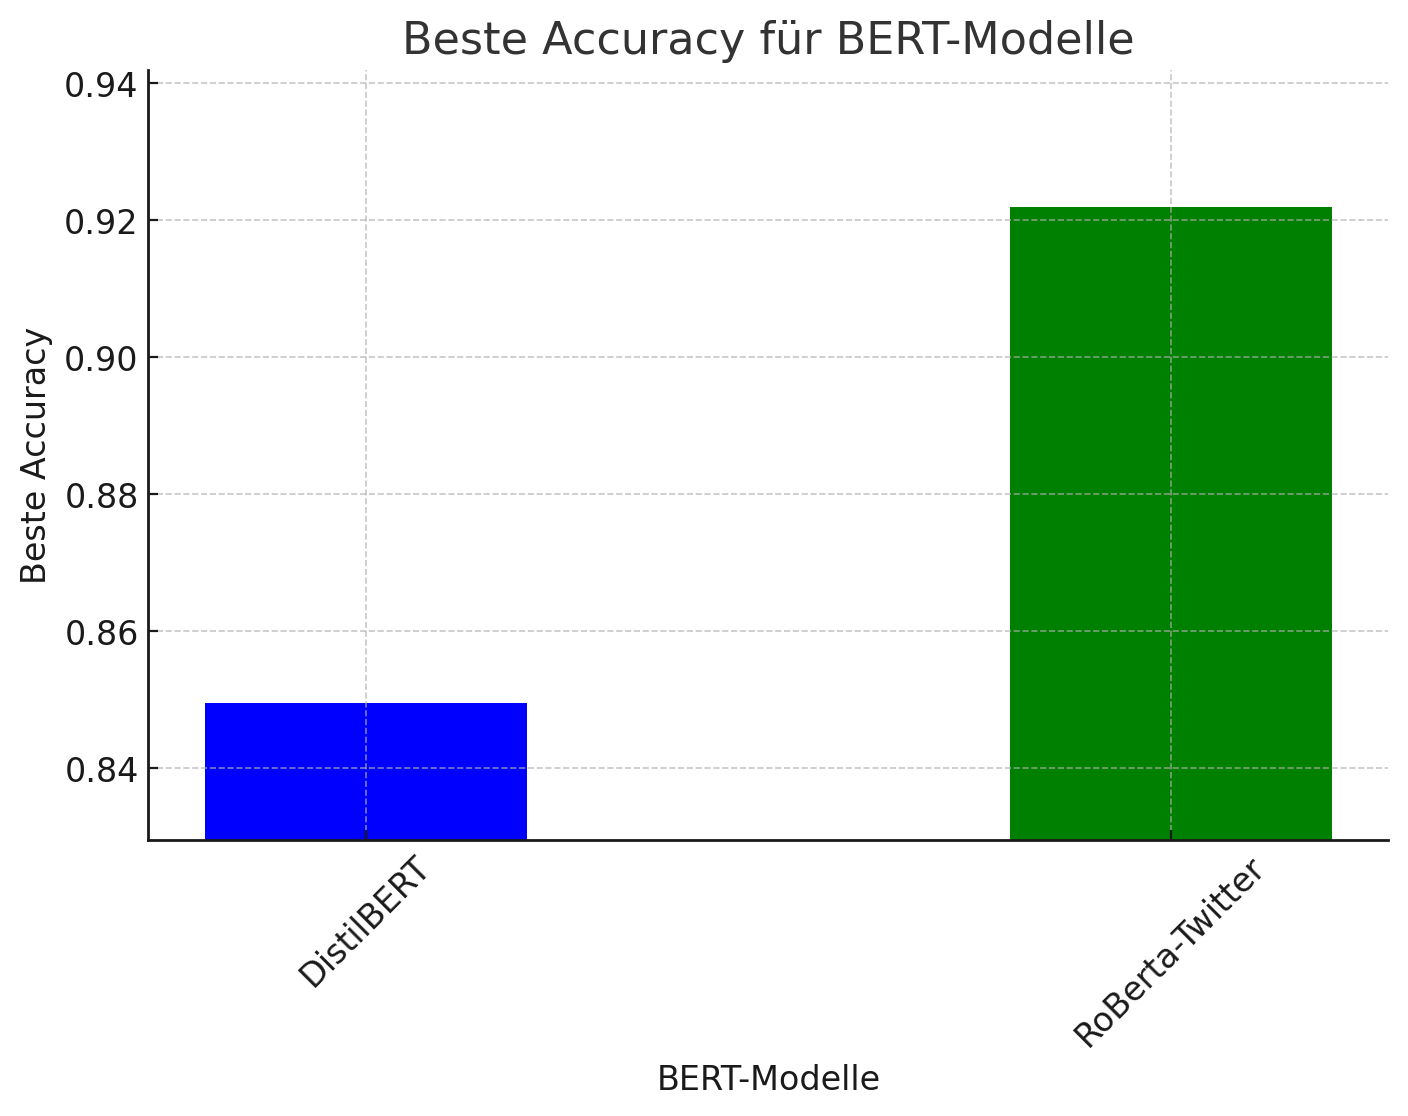
\includegraphics[scale=0.5]{bert.png}
\end{frame}

% BERT-basiert Modelle

% Erläuterung BERT-Modelle
% Fine-Tuning Ansatz
% Verwendet Modelle + Parameter
% Ergebnisse (jeweils ohne Fine-Tuning/Zero-Shot + Fine-Tuning)


% DeepSeek R1

% Modell-Erläuterung
% Fine-Tuning Ansatz lediglich erwähnen
% Verwendet Modelle + Prompt
% Ergebnisse (mit/ohne token-basierten Ansatz)
%  + Reasoning-Output

%distilbert-base-uncased
\begin{frame}{Ergebnisse}
    \centering
    \scriptsize
    \begin{tabular}{|l|l|l|l|}
        \hline
        \textbf{Modell} & \textbf{Daten-Größe} & \textbf{Lernrate} & \textbf{Test Accuracy} \\
        \hline
        DistilBERT & 20.000 & 0.0001 & 0.8496 \\
        RoBerta-Twitter & 20.000 & 0.0001 & 0.9220 \\
        \hline
    \end{tabular}
\end{frame}

\subsection{Fine-Tuning DeepSeek}
\begin{frame}{Fine-Tuning DeepSeek}
  \fontsize{10pt}{12pt}\selectfont
  \vspace{0.3cm}

  \begin{columns}
      % Linke Spalte: Modelle
      \column{0.45\textwidth}
      \textbf{DeepSeek-Modell}
      \vspace{0.3cm}
      \begin{itemize}
          \item \textbf{DeepSeek-R1-Distill-Qwen-1.5B}
      \end{itemize}
      \vspace{0.5cm}
      \textbf{Metrik:} Genauigkeit
      \vspace{-0.6cm}

      % Rechte Spalte: Parameterarten
      \column{0.55\textwidth}
      \textbf{Untersuchte Parameter}
      \vspace{0.3cm}
      \begin{itemize}
          \item \texttt{Initiale Lernrate}
          \item \texttt{Daten-Größe (Trainingsbeispiele)}
      \end{itemize}
  \end{columns}
\end{frame}

\begin{frame}{Ergebnisse}
    \centering
    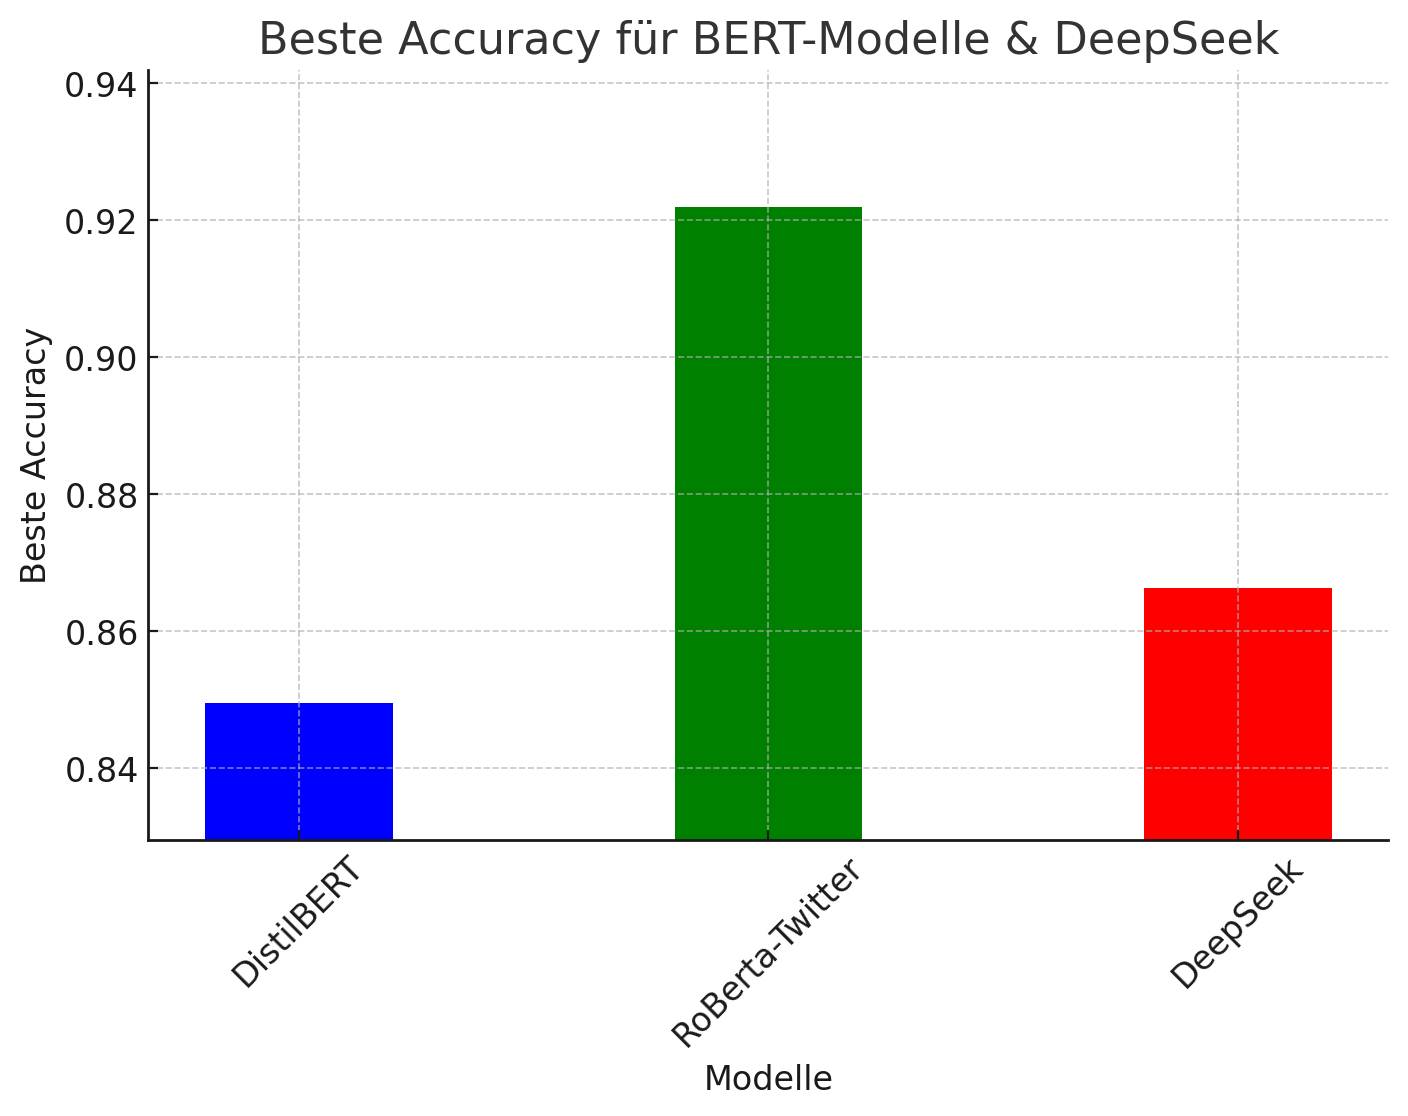
\includegraphics[scale=0.5]{bertdeepseek.png}
\end{frame}

\begin{frame}{Ergebnisse: BERT- und DeepSeek-Modelle}
    \centering
    \scriptsize
    \begin{tabular}{|l|l|l|l|}
        \hline
        \textbf{Modell} & \textbf{Daten-Größe} & \textbf{Lernrate} & \textbf{Test Accuracy} \\
        \hline
        DistilBERT & 20.000 & 0.0001 & 0.8496 \\
        RoBerta-Twitter & 20.000 & 0.0001 & 0.9220 \\
        DeepSeek & 20.000 & 0.0001 & 0.8663 \\
        \hline
    \end{tabular}
\end{frame}

\subsection{Zero-shot}
\begin{frame}{Zero-shot}
  \Large
  \textbf{Einschränkungen beim Fine-Tuning großer DeepSeek-Modelle:}

  \vspace{0.5cm}

  \begin{itemize}
      \item Fine-Tuning größerer \textbf{DeepSeek-Modelle} war aufgrund hoher Hardware-Anforderungen nicht möglich.
      \item Daher wurde für große DeepSeek-Modelle ein \textbf{Zero-Shot-Ansatz} gewählt.
      \item Modelle wurden ohne Training direkt auf Testdaten evaluiert.
      \item So konnte ihre Leistungsfähigkeit trotzdem verglichen werden.
  \end{itemize}

\end{frame}

\begin{frame}{Ergebnisse}
    \centering
    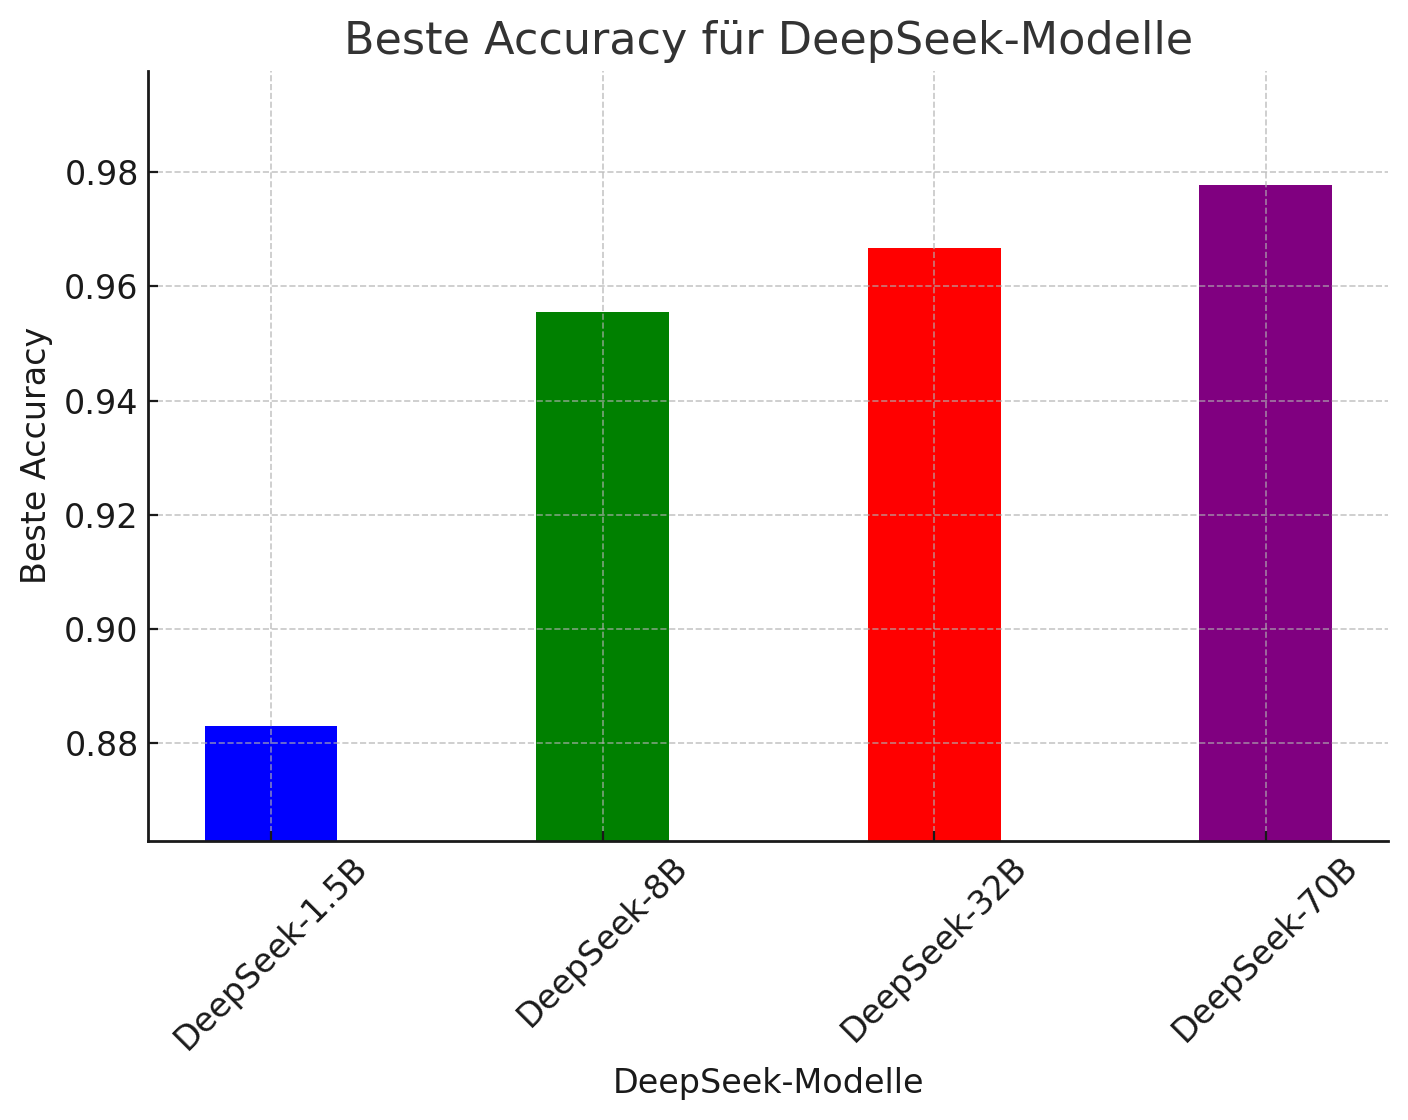
\includegraphics[scale=0.5]{deepseekzero.png}
\end{frame}

\begin{frame}{Ergebnisse}
    \centering
    \scriptsize
    \begin{tabular}{|l|l|l|}
        \hline
        \textbf{Modell} & \textbf{Mit Query-Term} & \textbf{Ohne Query-Term} \\
        \hline
        DeepSeek-1.5B & 0.8830 & 0.8245 \\
        DeepSeek-8B   & 0.9554 & 0.9164 \\
        DeepSeek-32B  & 0.9666 & 0.9276 \\
        DeepSeek-70B  & 0.9777 & 0.9304 \\
        \hline
    \end{tabular}
\end{frame}

\begin{frame}{Ergebnisse}
    \centering
    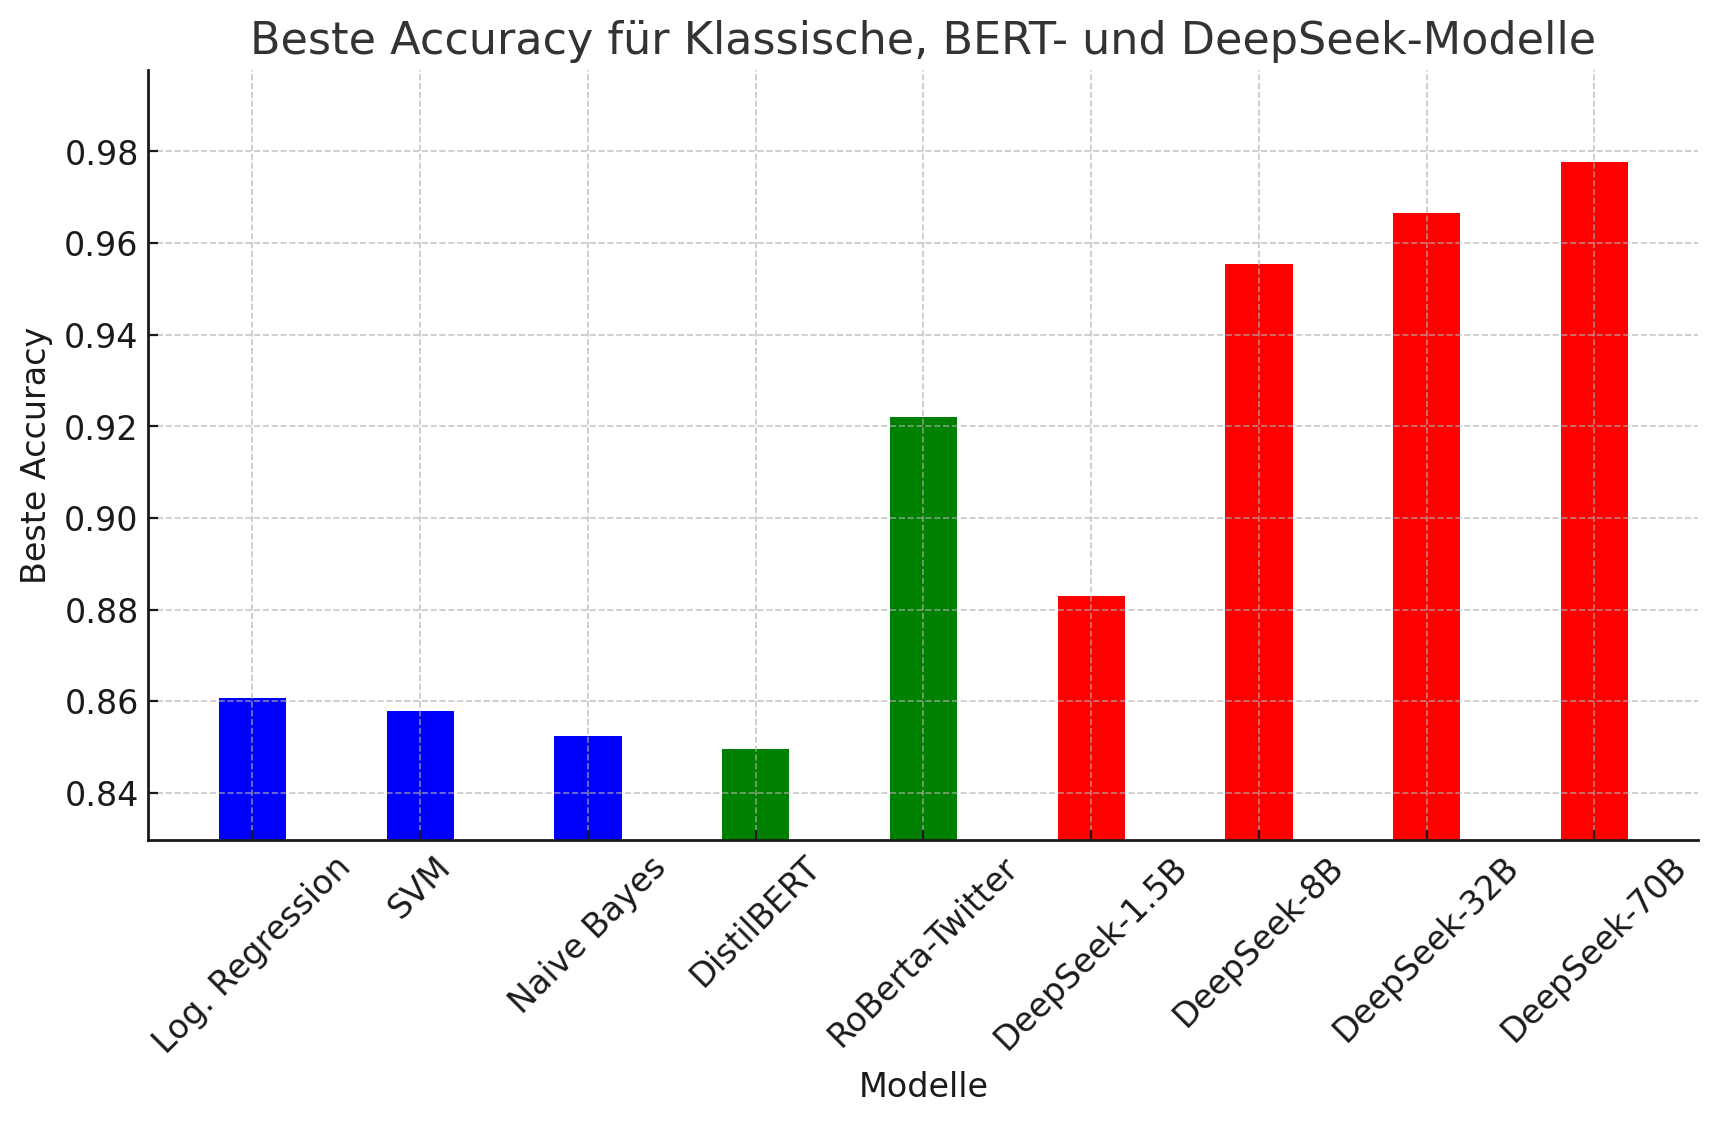
\includegraphics[scale=0.5]{all.png}
\end{frame}

%=========================================================================================================================
\section{Zusammenfassung}

% Stärkerer Fokus auf Ergebnisse
% - Vergleich der Modelle / Übersichts-Diagramm
% - Einschränkungen der einzelnen Modelle (Hardware, Trainingszeit)
\begin{frame}{Zusammenfassung}
  \normalsize
  \begin{itemize}
      \item Sentiment140-Datensatz gewählt und Tweets bereinigt
      \item Klassische Methoden trainiert und evaluiert
      \item BERT-Modell untrainiert evaluirt
      \item Fine-Tuning von BERT-Modellen durchgeführt
      \item DeepSeek-Modell mit Fine-Tuning getestet
      \item Zero-Shot-Ansatz für größere DeepSeek-Modelle verwendet
      \item Vergleich von Accuracy-Werten zwischen allen Modellen
      \item Skalierbarkeit und Hardware-Limits analysiert
      \item \textbf{Ausblick:}Größere DeepSeek-Modelle zeigen potenzial
  \end{itemize}

  \vspace{0.5cm}
  \centering
  \pause
  {\large \textbf{Vielen Dank für Ihre Aufmerksamkeit!}} \\[0.1cm]
  \textit{Fragen?}
\end{frame}

\end{document}
